\chapter{Multi-Cloud-Anwendungs-Broker}

Um eine Anwendung automatisiert auf verschiedene Clouds zu verteilen ist ein Broker-Mechanismus nötig. Dieser sollte nach verschiedenen, festzulegenden Kriterien vorgehen. Konkret erfüllt ein Broker in der Regel folgende Aufgaben:

\begin{enumerate}
	\item Bereitstellen der Ressourcen für eine Applikation; starten einer virtuellen Maschine oder Reservierung von Speicherplatz
	\item Starten der Anwendung auf den vorher reservierten Ressourcen
	\item Verteilen eingehender Anfragen auf die reservierten Ressourcen
	\item Management der Ressourcen
\end{enumerate}

\noindent In einer Community Cloud ist denkbar, dass die Cloud-Provider selbst einen Mechanismus zum Brokering oder zumindest offene APIs bereitstellen. Der Broker wäre also Teil der Cloud. Möglich sind entweder ein zentraler Broker, der direkt auf Cloud-Interna zugreift, aber auch ein Peer-to-Peer-Verbund.

Für Multi-Clouds kommen diese Lösungen nicht infrage: sie bestehen aus mehreren unabhängigen, meist privaten, Cloud-Providern. Aufgrund gegenläufiger Geschäftsinteressen sind diese nicht an einer Föderation mit anderen Anbietern interessiert. Sie werden also weder Interna ihrer Cloud-Plattform anpassen, noch einheitliche APIs bereitstellen.

Stattdessen muss der Broker in einer Multi-Cloud-Umgebung extern bereitgestellt werden. In diesem Fall kann er entweder als eigenständiger Service in Form einer \emph{Cloud Management Platform} angelegt sein, oder von der verteilten Anwendung selbst implementiert werden. Selbst entwickelte CMPs oder integrierte Broker setzen oft auf Multi-Cloud-Bibliotheken wie Apache libcloud. Kapitel \todo{Link} bietet dazu einen Vergleich. 

Zusätzlich sollte der Multi-Cloud-Broker Policys auswerten und umsetzen können. Der folgende Abschnitt gibt eine Übersicht der bisherigen Forschung zu Inter- und Multi-Cloud-Brokern sowie Cloud Management Plattformen.

\section{Related Work}

Die vorgestellten Lösungen unterschieden sich in Architektur, Flexibilität und Funktionsumfang. Die vier Basiseigenschaften werden nicht von allen Arbeiten in vollem Umfang erfüllt. Zusätzlich denkbar ist das automatische Re-provisionieren anhand von 

\begin{enumerate}
	\item Lastspitzen oder Ausfällen von Hardware und Netzwerkressourcen (Monitoring)
	\item Geänderten Umfeldparametern wie der Gesetzgebung, Preise oder AGBs
	\item Nutzeränderungen
	\item Vorherigen Broker-Aktionen
\end{enumerate}

policy-driven service placement optimization in federated clouds 



\begin{description}
	\item[ManageIQ] Kommerzielle Cloud Management Platform, unterstützt alle wichtigen IaaS-Provider (AWS, Azure, GCP, OpenStack. Besonderheit: )
\end{description}

ManageIQ commercial
- policies! Conditions, Actions, Profiles
%http://manageiq.org/docs/reference/latest/doc-Policies_and_Profiles_Guide/miq/


Commercial (Rightscale) 

only trigger-action, no SLAs 

Apache Scalr (complex, freemium) 





RESERVOIR (hard and soft requirements) 



OPTIMIS (Trust/Risk/Eco/Cost) 

canceled research project 

Dependable sociability = trust + risk + eco + cost 

introducing new multi-cloud HYBRID architectures with broker 

combination of federation and multi-cloud 

no geo-location 

non-disclosed algorithm 

no current external adapter available 

SP and IP, focus on IP benefit 





Contrail 

Federation 

Meta-data access (location, price..) 

although not usable in SLAs  :( 



Meryn 

SLA-driven PaaS system 

Optimize Cloud Provider costs 

Cloud Bursting 

Batch-application-centered (Hadoop) 

Single-use VMs 

Bidding 



InterCloud 

Pricing-aware 

Broker 

Federation 



Seaclouds EU project 

2013 

Cloud agnostic PaaS 

Discover/Planner/Deploy/Monitor/SLA-Services 

only monitors user-specific SLA 

Not used during planning/matchmaking 



Mist.io 

Open source 

Build on libcloud and cloudify 

Can monitor costs (commercial) 

No automatic scheduling 



DivvyCloud (Commercial) 

Automation Bots to schedule downtime, terminate, or re-size instances and resources so you only pay for what you use 

https://divvycloud.com/product/botfactory/for-cost/ 


An SLA-based Broker for Cloud Infrastructures 



Nicht nur Private Clouds sondern auch Personal Devices 



Modulare Architektur 



Fokus auf Föderation. Aber: Idee der forced integration of commercial cloud providers 

-> Mithilfe libcloud umsetzen 


\section{Architektur}

Komponenten des Brokers.


In der CMP: Polling oder Notification?

Was löst eine Aktion aus?
- Monitoring der Services
- Änderung der Umgebung
- User-Aktion
- Ergebnis einer anderen Policy

\begin{figure}
	\centering
	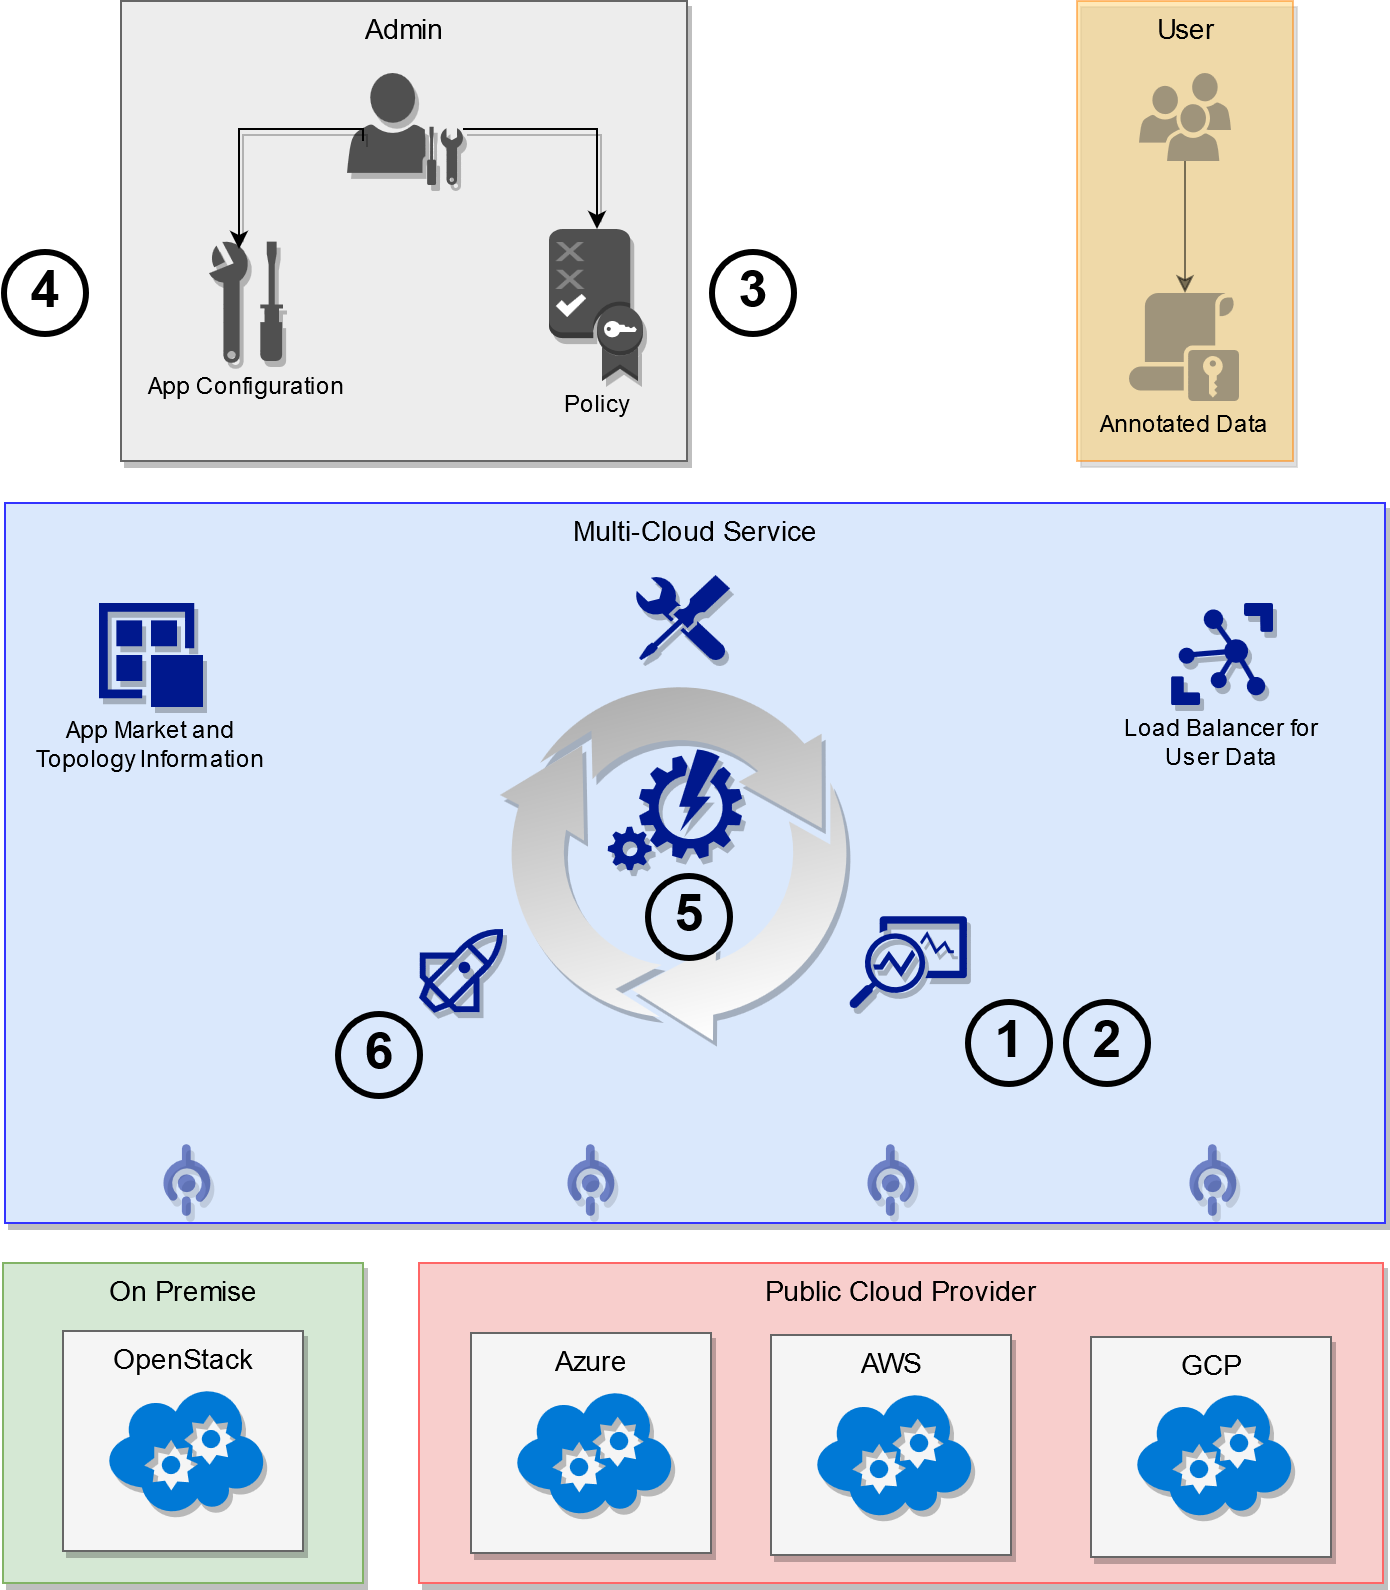
\includegraphics[width=0.9\linewidth]{images/cycle}
	\caption{}
	\label{fig:Chicken1}
\end{figure}

Zyklus\autoref{fig:Chicken1}:

%\begin{description}
%	\item[Nummerierte Aufzählung]~\par
\begin{enumerate}
	
	\item Sammeln der Meta-Informationen alle Cloud-Provider
	\begin{enumerate}
		\item Kapazität (CPU, RAM, HDD, Network)
		\item Features (Verschlüsselung, CUDA, …)
		\item Geo-Lokation 
		\item Preis
	\end{enumerate}
	
	\item Sammeln der Laufzeitinformationen der PaaS/Anwendungen
	\begin{enumerate}
		\item Auslastung
		\item Fehler
		\item Ausfälle
	\end{enumerate}
	
	\item Sammeln der SLAs
	\begin{enumerate}
		\item Policy-Definitionen
		\item Policy-Konfiguration
		\item Placement-Algorithmen
	\end{enumerate}

	\item Neue Anwendung/Änderung eines SLA
	
	\item Optimierung
	\begin{enumerate}
		\item Feste Vorgaben (Geo, Backup)
		\item Weiche (Preis, Latenz, Verfügbarkeit)
	\end{enumerate}

	
	\item Ausführung
	\begin{enumerate}
		\item Netzwerkkonfiguration
		\item Allokation/De-Allokation von Ressourcen
		\item Deployment
		\item Migration
		\item Logging/Benachrichtigung
		\item Backup
	\end{enumerate}

\end{enumerate}
%\end{description} 

\section{Schemata: Cloud-Angebote, SLAs, Services}

\section{Matching}
%
%Angebot der Cloud Provider (SLA)
%Anforderungen
%
%Spezifizierung
%Schnittstellen
%
%Algorithmen